\documentclass[10pt]{beamer}
\usefonttheme{professionalfonts,serif}
\def\newblock{\hskip .11em plus .33em minus .07em}
\usepackage[numbers,sort]{natbib}
\renewcommand{\rmdefault}{psbx}
\usepackage[utf8]{inputenc}
\usepackage[T1]{fontenc}
\usepackage{textcomp}
\usepackage{eulervm}

\usetheme{default}           % tips from David Blei
\useinnertheme{circles}
\useoutertheme{infolines}
\setbeamertemplate{headline}{}
\setbeamertemplate{navigation symbols}{}
\setbeamerfont{itemize/enumerate subbody}{size=\normalsize}
\setbeamerfont{itemize/enumerate subsubbody}{size=\normalsize}
\usecolortheme{seahorse}
\setbeamersize{text margin left=2mm,text margin right=2mm}

\graphicspath{{../../figures/}}

\definecolor{mypine}{rgb}{0.05,0.45,0.05}
\definecolor{mycyan}{rgb}{0.0,0.9,0.9}
\newcommand{\Red}{\textcolor{red}}
\newcommand{\Blue}{\textcolor{blue}}
\newcommand{\Green}{\textcolor{mypine}}
\newcommand{\PineGreen}{\textcolor{mypine}}
\newcommand{\Magenta}{\textcolor{magenta}}
\newcommand{\Cyan}{\textcolor{mycyan}}

\newcommand{\N}{\mathcal{N}}
\newcommand{\R}{\mathbb{R}}
\newcommand{\T}{{\scriptsize^{\top}}}
\newcommand{\D}{\mathcal{D}}
\newcommand{\F}{\mathcal{F}}
\newcommand{\E}{\mathbb{E}}
\newcommand{\V}{\mathbb{V}}
\newcommand{\M}{\mathcal{M}}
\newcommand{\KL}{\mathcal{KL}}
\newcommand{\cut}[1]{}
\newcommand{\trace}{\operatorname{trace}}

\newcommand{\bmu}{{\boldsymbol{\mu}}}
\newcommand{\btheta}{\boldsymbol{\theta}}
\newcommand{\bepsilon}{\boldsymbol{\epsilon}}
\newcommand{\balpha}{\boldsymbol{\alpha}}
\newcommand{\bbeta}{\boldsymbol{\beta}}
\newcommand{\bphi}{\boldsymbol{\phi}}
\newcommand{\bPhi}{\boldsymbol{\Phi}}
\newcommand{\bSigma}{\boldsymbol{\Sigma}}
\newcommand{\bpi}{\boldsymbol{\pi}}
\newcommand{\blambda}{\boldsymbol{\lambda}}

\newcommand{\argmax}{\operatorname{argmax}}
\newcommand{\argmin}{\operatorname{argmin}}
\newcommand{\ci}{{\bot\negthickspace\negthickspace\bot}} % conditional indep.
\newcommand{\neigh}{\operatorname{ne}}
\newcommand{\vectr}[2]{  \left[ \!\!\begin{array}{c} #1 \\
      #2 \end{array} \!\!\right]}
\newcommand{\deff}{\stackrel{\mathrm{def}}{=}}
\newcommand{\deldel}[2]{\frac{\partial #1}{\partial #2}}

\newcommand{\maketilde}{\raisebox{0.4ex}{\tiny $\sim$}}
\newcommand{\bfa}{\mathbf a}
\newcommand{\bfb}{\mathbf b}
\newcommand{\bfe}{\mathbf e}
\newcommand{\bff}{\mathbf f}
\newcommand{\bfk}{\mathbf k}
\newcommand{\bfm}{\mathbf m}
\newcommand{\bfn}{\mathbf n}
\newcommand{\bfp}{\mathbf{p}}
\newcommand{\bfs}{\mathbf s}
\newcommand{\bfu}{\mathbf u}
\newcommand{\bfx}{\mathbf x}
\newcommand{\bfy}{\mathbf y}
\newcommand{\bft}{\mathbf t}
\newcommand{\bfv}{\mathbf v}
\newcommand{\bfw}{\mathbf w}
\newcommand{\bfA}{\mathbf A}
\newcommand{\bfI}{\mathbf I}
\newcommand{\bfK}{\mathbf K}

\usepackage{bbm}

\title{Latent Dirichlet Allocation for Topic Modeling}
\author{Carl Edward Rasmussen}
\date{November 18th, 2016}

\begin{document}


\begin{frame}
\titlepage
\end{frame}

\cut{
\begin{frame}
\frametitle{Key concepts}

\begin{itemize}
\item fitting the mixture model with EM
\end{itemize}
\end{frame}
}

\begin{frame}
\frametitle{Limitations of the mixture of categoricals model}

\begin{minipage}{0.7\linewidth}
\centerline{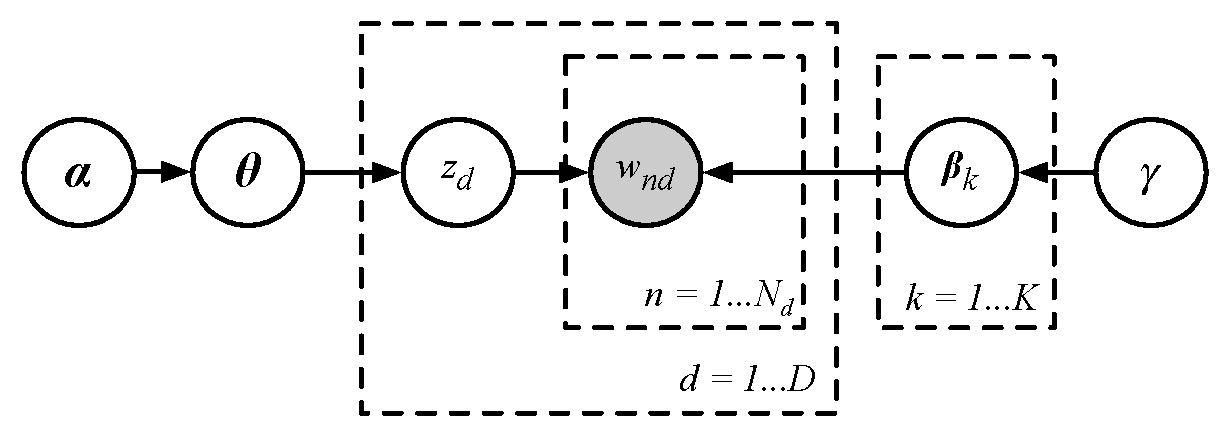
\includegraphics[width=0.9\textwidth]{bayes_mix_categorical_model}}
\end{minipage}
\begin{minipage}{0.29\linewidth}
\begin{eqnarray*}
\btheta & \sim& {\rm{Dir}}(\alpha)\\
\bbeta_k & \sim &{ \rm{Dir}}(\gamma)\\
z_d & \sim & \rm{Cat}(\btheta)\\
w_{nd} | z_d & \sim & \rm{Cat}(\bbeta_{z_d})
\end{eqnarray*}
\end{minipage}


A generative view of the mixture of categoricals model
\begin{enumerate}
\item Draw a distribution $\btheta$ over $K$ topics from a Dirichlet($\alpha$).
\item For each topic $k$, draw a distribution $\bbeta_k$ over words from a
  Dirichlet($\gamma$).
\item For each document $d$, draw a topic $z_d$ from a Categorical($\btheta$)
\item For each document $d$, draw $N_d$ words $w_{nd}$ from a Categorical($\bbeta_{z_d}$)
\end{enumerate}

Limitations:
\begin{itemize}
\item All words in each document are drawn from one specific topic distribution.
\item This works if each document is exclusively about one topic, but if 
some documents span more than one topic, then ``blurred'' topics must be
learnt.
\end{itemize}

\end{frame}


\begin{frame}
\frametitle{NIPS dataset: LDA topics 1 to 7 out of 20.}

{\scriptsize
\begin{tabular}{l l l l l l l} 
network & network & model & problem & neuron & network & cell\\ 
unit & node & data & constraint & cell & neural & model\\ 
training & representation & distribution & distance & input & system & visual\\ 
weight & input & probability & cluster & model & model & direction\\ 
input & unit & parameter & point & synaptic & control & motion\\ 
hidden & learning & set & algorithm & firing & output & field\\ 
output & activation & gaussian & tangent & response & recurrent & eye\\ 
learning & nodes & error & energy & activity & input & unit\\ 
layer & pattern & method & clustering & potential & signal & cortex\\ 
error & level & likelihood & optimization & current & controller & orientation\\ 
set & string & prediction & cost & synapses & forward & map\\ 
neural & structure & function & graph & membrane & error & receptive\\ 
net & grammar & mean & method & pattern & dynamic & neuron\\ 
number & symbol & density & neural & output & problem & input\\ 
performance & recurrent & prior & transformation & inhibitory & training & head\\ 
pattern & system & estimate & matching & effect & nonlinear & spatial\\ 
problem & connectionist & estimation & code & system & prediction & velocity\\ 
trained & sequence & neural & objective & neural & adaptive & stimulus\\ 
generalization & order & expert & entropy & function & memory & activity\\ 
result & context & bayesian & set & network & algorithm & cortical
\end{tabular}
}
\end{frame}


\begin{frame}
\frametitle{NIPS dataset: LDA topics 8 to 14 out of 20.}

{\scriptsize
\begin{tabular}{l l l l l l l} 
circuit & learning & speech & classifier & network & data & function\\ 
chip & algorithm & word & classification & neuron & memory & linear\\ 
network & error & recognition & pattern & dynamic & performance & vector\\ 
neural & gradient & system & training & system & genetic & input\\ 
analog & weight & training & character & neural & system & space\\ 
output & function & network & set & pattern & set & matrix\\ 
neuron & convergence & hmm & vector & phase & features & component\\ 
current & vector & speaker & class & point & model & dimensional\\ 
input & rate & context & algorithm & equation & problem & point\\ 
system & parameter & model & recognition & model & task & data\\ 
vlsi & optimal & set & data & function & patient & basis\\ 
weight & problem & mlp & performance & field & human & output\\ 
implementation & method & neural & error & attractor & target & set\\ 
voltage & order & acoustic & number & connection & similarity & approximation\\ 
processor & descent & phoneme & digit & parameter & algorithm & order\\ 
bit & equation & output & feature & oscillation & number & method\\ 
hardware & term & input & network & fixed & population & gaussian\\ 
data & result & letter & neural & oscillator & probability & network\\ 
digital & noise & performance & nearest & states & item & algorithm\\ 
transistor & solution & segment & problem & activity & result & dimension
\end{tabular}
}

\end{frame}


\begin{frame}
\frametitle{NIPS dataset: LDA topics 15 to 20 out of 20.}

{\scriptsize
\begin{tabular}{l l l l l l l} 
function & learning & model & image & rules & signal\\ 
network & action & object & images & algorithm & frequency\\ 
bound & task & movement & system & learning & noise\\ 
neural & function & motor & features & tree & spike\\ 
threshold & reinforcement & point & feature & rule & information\\ 
theorem & algorithm & view & recognition & examples & filter\\ 
result & control & position & pixel & set & channel\\ 
number & system & field & network & neural & auditory\\ 
size & path & arm & object & prediction & temporal\\ 
weight & robot & trajectory & visual & concept & model\\ 
probability & policy & learning & map & knowledge & sound\\ 
set & problem & control & neural & trees & rate\\ 
proof & step & dynamic & vision & information & train\\ 
net & environment & hand & layer & query & system\\ 
input & optimal & joint & level & label & processing\\ 
class & goal & surface & information & structure & analysis\\ 
dimension & method & subject & set & model & peak\\ 
case & states & data & segmentation & method & response\\ 
complexity & space & human & task & data & correlation\\ 
distribution & sutton & inverse & location & system & neuron
\end{tabular}
}

\end{frame}


\begin{frame}
\frametitle{Latent Dirichlet Allocation (LDA)}

\centerline{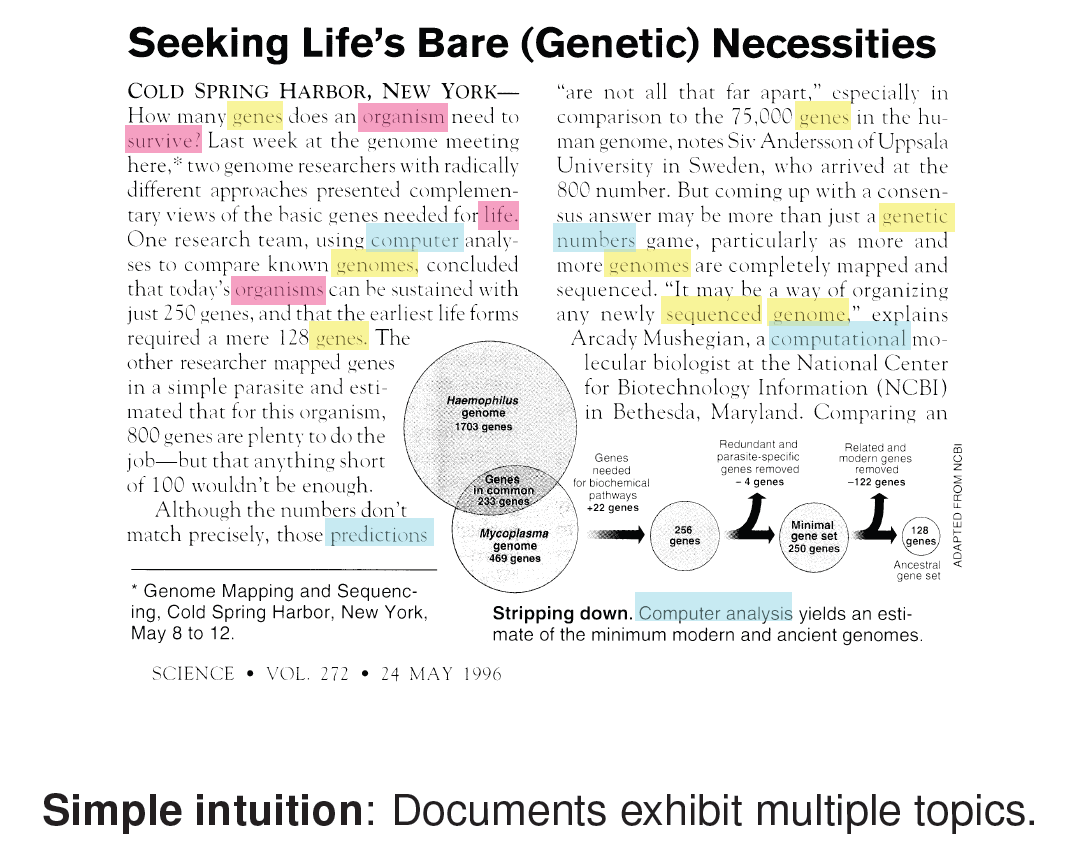
\includegraphics[width=\textwidth]{LDA_toy_graph1}}

Simple intuition (from David Blei): Documents exhibit multiple topics.

\end{frame}


\begin{frame}
\frametitle{Generative model for LDA}

\centerline{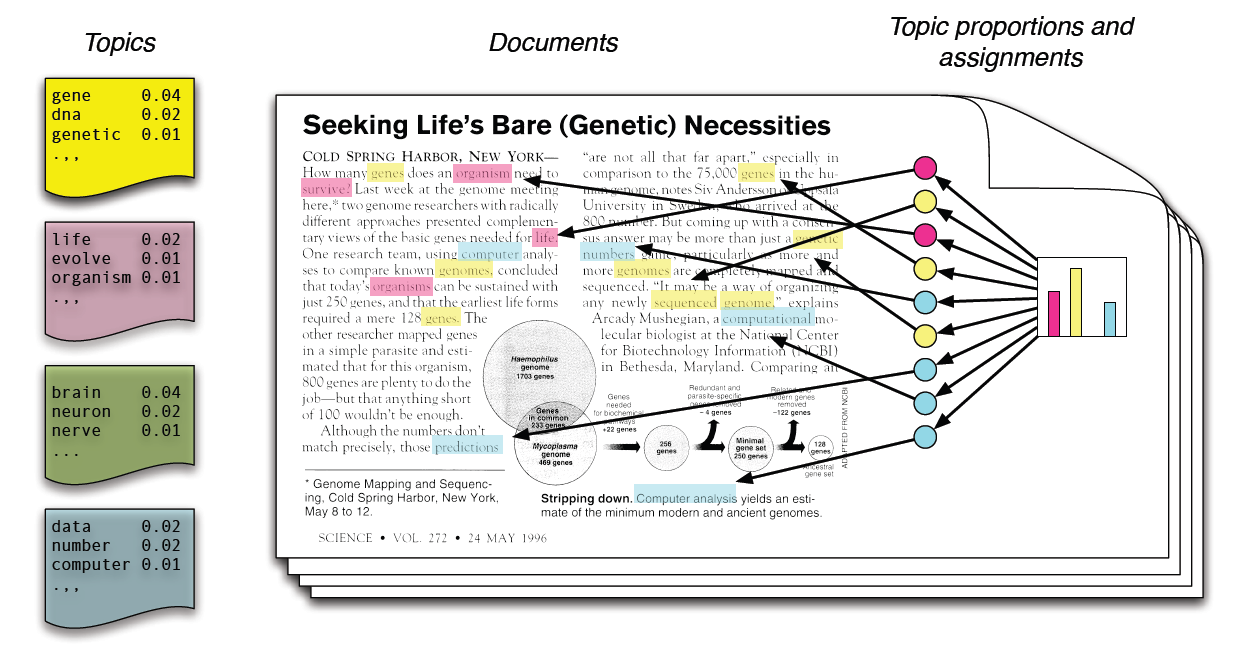
\includegraphics[width=\textwidth]{LDA_toy_graph2}}

\begin{itemize}
\item Each \Blue{\emph{topic}} is a distribution over words.
\item Each \Blue{\emph{document}} is a mixture of corpus-wide topics.
\item Each \Blue{\emph{word}} is drawn from one of those topics.
\end{itemize}
\hfill{\tiny from David Blei}
\end{frame}


\begin{frame}
\frametitle{The posterior distribution}

\centerline{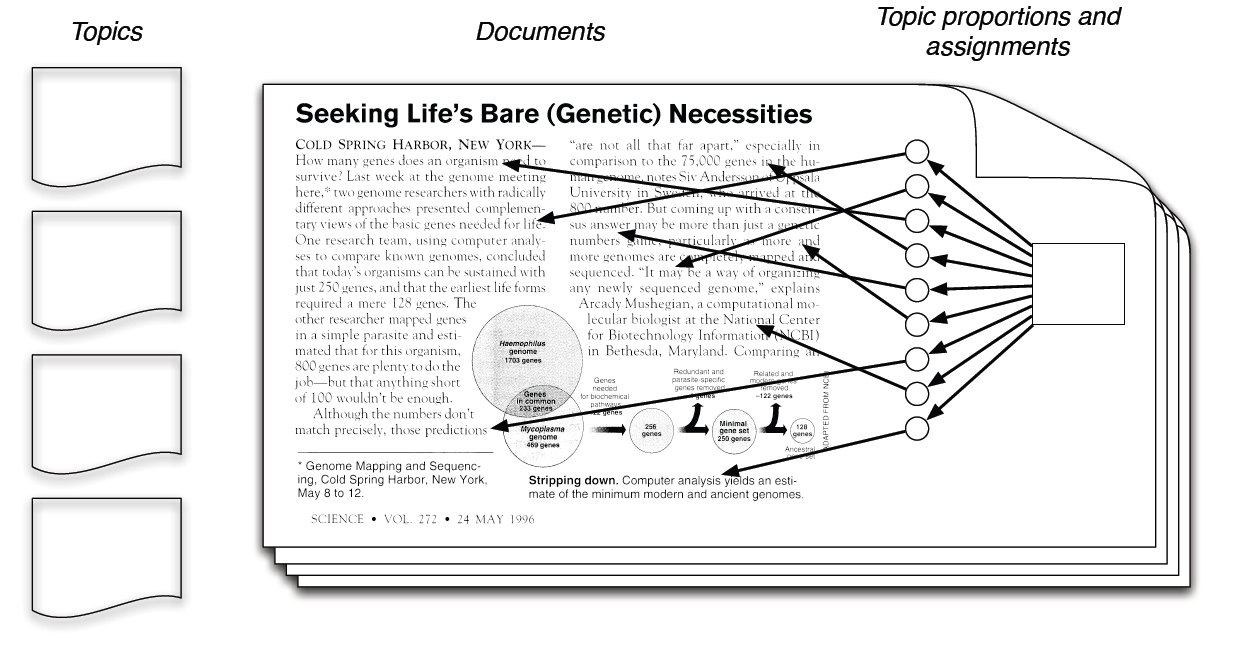
\includegraphics[width=\textwidth]{LDA_toy_graph3}}
\begin{itemize}
\item In reality, we only observe the documents.
\item The other structure are \Blue{\emph{hidden}} variables.
\end{itemize}
\hfill{\tiny from David Blei}
\end{frame}


\begin{frame}
\frametitle{The posterior distribution}

\centerline{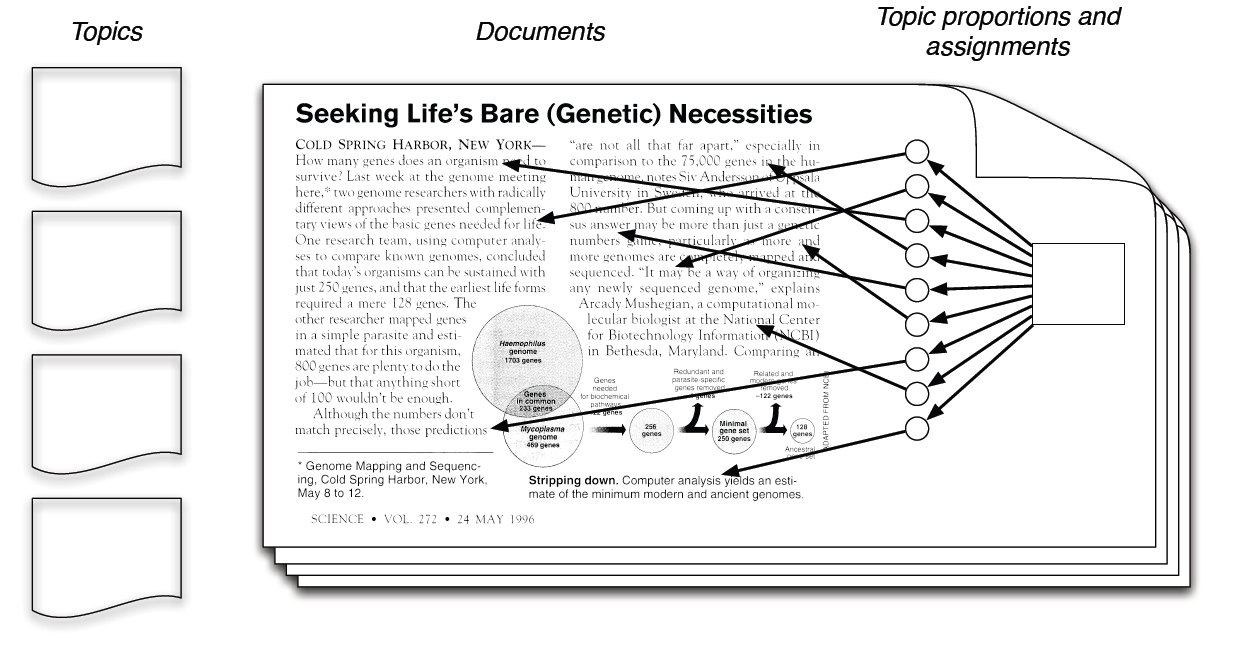
\includegraphics[width=\textwidth]{LDA_toy_graph3}}
\begin{itemize}
\item Our goal is to \Blue{\emph{infer}} the hidden variables.
\item This means computing their distribution conditioned on the documents
\centerline{p(topics, proportions, assignments|documents)}
\end{itemize}
\hfill{\tiny from David Blei}

\end{frame}


\begin{frame}
\frametitle{The LDA graphical model}

\centerline{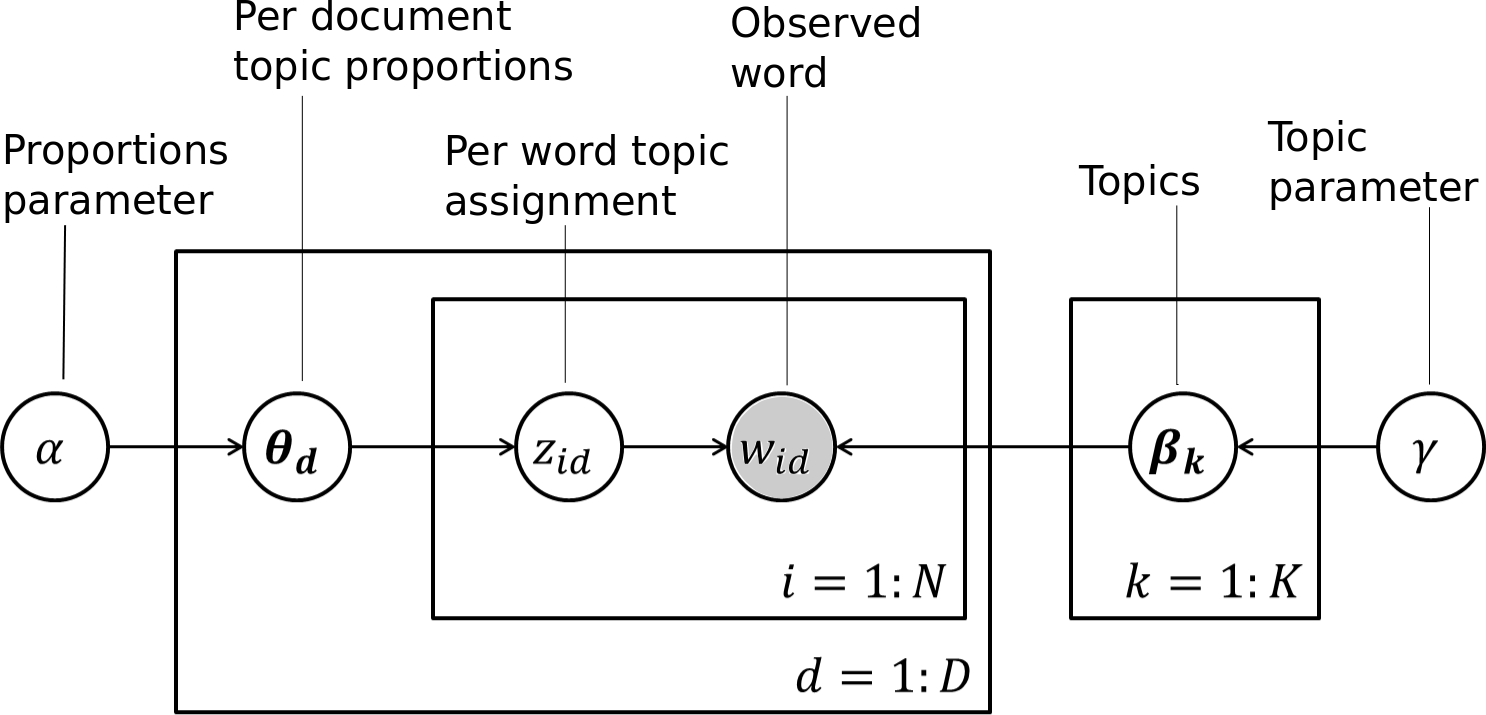
\includegraphics[width=0.8\textwidth]{LDA_model_annotated}}

\begin{itemize}
\item Nodes are random variables; edges indicate dependence.
\item Shaded nodes indicate \Blue{\emph{observed}} variables.
\end{itemize}

\end{frame}


\begin{frame}
\frametitle{The difference between mixture of categoricals and LDA}

\centerline{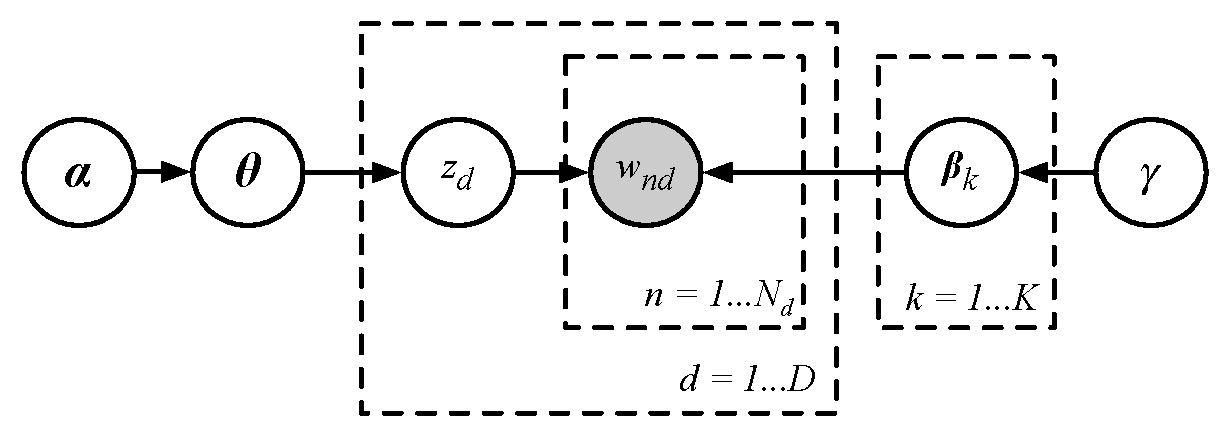
\includegraphics[width=0.45\textwidth]{bayes_mix_categorical_model}\hspace*{2ex}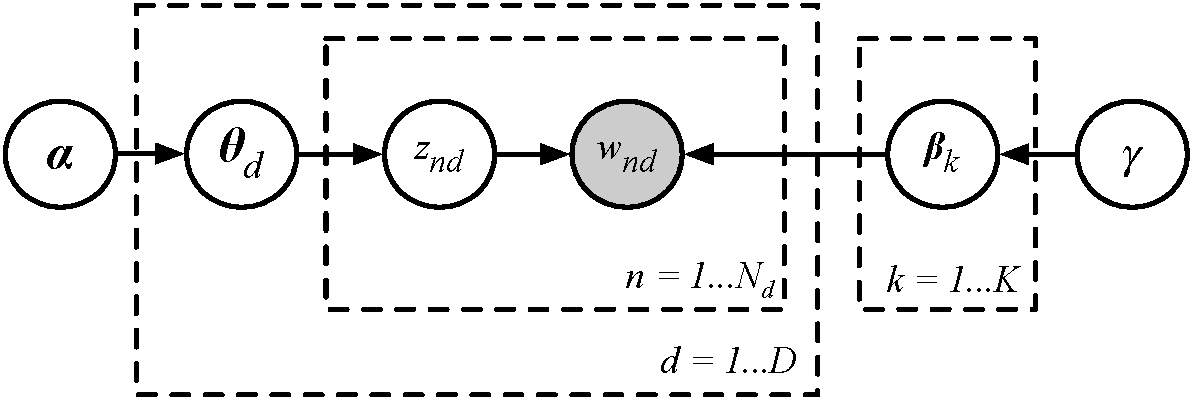
\includegraphics[width=0.45\textwidth]{lda2}}

A generative view of LDA
\begin{enumerate}
\item For each document $d$ draw a distribution $\btheta_d$ over
  topics from a Dirichlet($\alpha$).
\item For each topic $k$ draw a distribution $\bbeta_k$ over words
  from a Dirichlet($\gamma$). 
\item Draw a topic $z_{nd}$ for the $n$-th word in document $d$ from a
  Categorical($\btheta_d$)
\item Draw word $w_{nd}$ from a Categorical($\bbeta_{z_{nd}}$)
\end{enumerate}

Differences with the mixture of categoricals model:
\begin{itemize}
\item In LDA, every word in a document can be drawn from a different
  topic, 
\item and every document has its own distribution over topics $\btheta_d$.
\end{itemize}

\end{frame}


\begin{frame}
\frametitle{The LDA inference problem}

\centerline{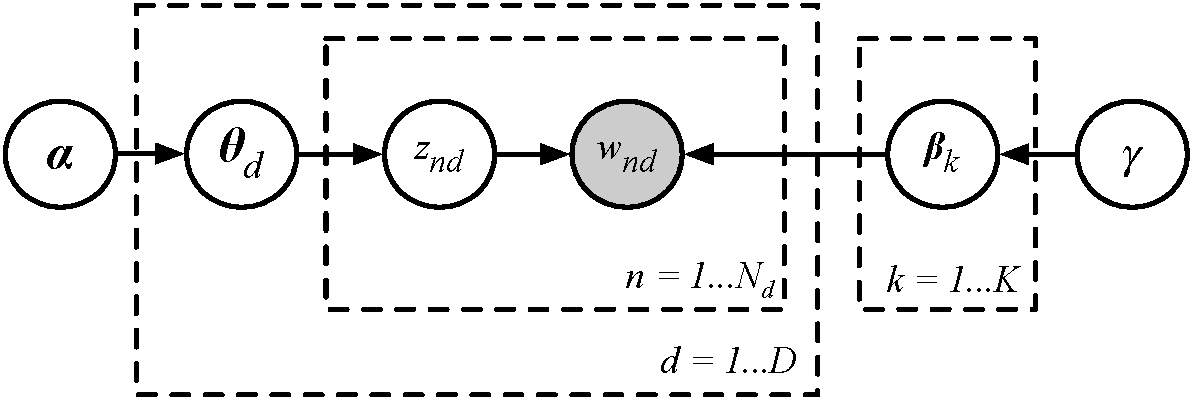
\includegraphics[width=0.5\textwidth]{lda2}}

\emph{``Always write down the probability of everything.''} (Steve Gull)
%
\begin{align*}
p(\bbeta_{1:K},\btheta_{1:D},\{z_{nd}\}&,\{w_{nd}\}|\gamma, \alpha)\\
&=\prod_{k=1}^K p(\bbeta_k|\gamma) \; \prod_{d=1}^D \left[ p(\btheta_d|\alpha)
\prod_{n=1}^{N_d} \big[
p(z_{nd}|\btheta_d)p(w_{nd}|\bbeta_{1:K},z_{nd})\big] \right]
\end{align*}
%

Learning involves computing the posterior over the parameters, $\bbeta_{1:K}$ and
$\btheta_{1:D}$ given the words $\{w_{nd}\}$, but this requires the we
marginalize out the latent $\{z_{nd}\}$.\\[1ex]

How many configurations are there?\\[1ex]

This computation is \Blue{\emph{intractable}}.

\cut{
The posterior of interest is given by
%
\begin{align*}
p(\bbeta_{1:K},\btheta_{1:D},\{z_{nd}\}|\{w_{nd}\}|\gamma, \alpha)=
\frac{p(\bbeta_{1:K},\btheta_{1:D},\{z_{nd}\},\{w_{nd}\}|\gamma, \alpha)}{p(\{w_{id}\})}
\end{align*}
%

But it is \Blue{\emph{intractable}} because we cannot compute the evidence $p(\{w_{nd}\})$.
}
\end{frame}


\begin{frame}
\frametitle{The intractability of LDA}

The evidence (normalising constant of the posterior):
%
\[
p(\{w_{id}\})=
\int\int
\sum_{z_{id}}
\prod_{d=1}^D \prod_{k=1}^K
\prod_{n=1}^{N_d} 
 p(z_{nd}|\btheta_d)p(\btheta_d|\alpha)
 p(w_{nd}|\bbeta_{1:K},z_{nd})p(\bbeta_k|\gamma)\mathrm{d}\bbeta_k\mathrm{d}\btheta_d
\]
%

We need to average over all possible set of values of all $z_{nd}$. If
every document had $N$ words, this means $K^N$ configurations per document.

\end{frame}


\begin{frame}
\frametitle{Gibbs to the Rescue}

The posterior is \emph{\Blue{intractable}} because there are \Red{too many}
possible latent $\{z_{nd}\}$.\\[1ex]

Sigh, $\ldots$ if only we knew the $\{z_{nd}\}$ $\ldots$?\\[1ex]

Which might remind us of Gibbs sampling $\ldots$ could we sample 
each latent variable given the values of the other ones?

\end{frame}


\begin{frame}
\frametitle{Refresher on Beta and Dirichlet}

If we had a $p(\pi) = \operatorname{Beta}(\alpha,\beta)$ prior on a \Blue{binomial}
probability $\pi$,  and observed $k$ successes and $n-k$ failures, then the
posterior probability 
\[
p(\pi|n,k) = \operatorname{Beta}(\alpha+k,\beta+n-k),
\]
and the predictive probability of success at the next experiment
\[
p(\mathrm{success}|n,k) = \int p(\mathrm{success}|\pi) p(\pi| n,k)  d\pi = \E[\pi|n,k]\;=\;\frac{\alpha+k}{\alpha+\beta+n}.
\]

\centerline{\rule{0.5\textwidth}{.4pt}}

Analogously, if we had a
prior $p(\boldsymbol{\pi}) = \operatorname{Dir}(\alpha_1,\ldots,\alpha_k)$ on the parameter
$\boldsymbol{\pi}$ of a \Blue{multinomial}, and $c_1,\ldots,c_k$
observed counts of each value, the posterior is
\[
p(\boldsymbol\pi| c_1,\ldots,c_k) =  \operatorname{Dir}(\alpha_1+c_1,\ldots,\alpha_k+c_k),
\]
and the predictive probability that the next item takes value $j$ is:
\[
p(j|c_1,\ldots,c_k) = \int p(j|\boldsymbol\pi)
p(\boldsymbol\pi|c_1,\ldots,c_k) d\boldsymbol\pi =
\E[\boldsymbol\pi|c_1,\dots,c_k] \;=\;\frac{\alpha_j+c_j}{\sum_i\alpha_i+c_i}.
\]

\end{frame}


\begin{frame}
\frametitle{Collapsed Gibbs sampler for LDA}

In the LDA model, we can integrate out the parameters of the multinomial
distributions, $\theta_d$ and $\beta$, and just keep the latent counts
$z_{nd}$. Sampling these $z_{nd}$ in turn is called a
\Blue{\emph{collapsed}} Gibbs sampler. 

Recall, that the predictive distribution for a symmetric Dirichlet is given by
\[
p_i\;=\;\frac{\alpha+c_i}{\sum_j \alpha + c_j}.
\]

Now, for Gibbs sampling, we need the predictive distribution for a
single $z_{nd}$ given all other $z_{nd}$, ie, given all the counts
except for the word $n$ in document $d$.\\
The Gibbs update contains two parts, one from the topic distribution
and one from the word distribution:
\[
p(z_{nd}=k|\{z_{-nd}\}, \{w\},\gamma, \alpha) \;\propto\;
 \frac{\alpha+c_{-nd}^k}{\displaystyle \sum_{j=1}^K (\alpha + c_{-nd}^j)} \;\;\;
\frac{\gamma + \tilde{c}_{-w_{nd}}^k}{\displaystyle \sum_{m=1}^M (\gamma +
  \tilde{c}_{-m}^k)}
\]
where $c^k_{-nd}$ is the count of words from document $d$, excluding
$n$, assigned 
to topic $k$, and  $\tilde{c}_{-m}^k$ is the number of times word $m$
was generated from topic $k$ (again, excluding the observation $nd$).
\end{frame}


\begin{frame}
\frametitle{Derivation of the collapsed Gibbs sampler}

\centerline{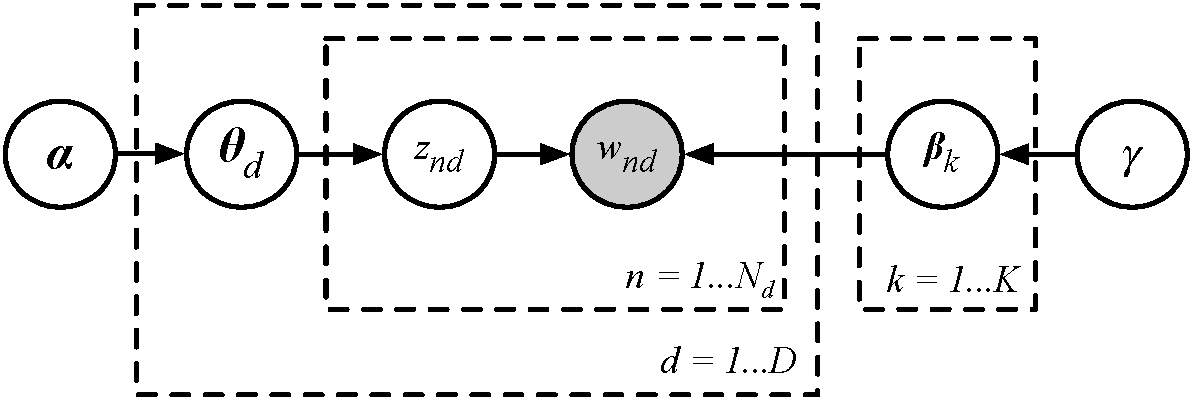
\includegraphics[width=0.4\textwidth]{lda2}}

The probability of everything:
{\small
\begin{align*}
p(\bbeta_{1:K},\btheta_{1:D},\{z_{nd}\},\{w_{nd}\}|\gamma, \alpha)
=\prod_{k=1}^K p(\bbeta_k|\gamma) \; \prod_{d=1}^D \left[ p(\btheta_d|\alpha)
\prod_{n=1}^{N_d} \big[
p(z_{nd}|\btheta_d)p(w_{nd}|\bbeta_{1:K},z_{nd})\big] \right]
\end{align*}
}
What we want for Gibbs sampling is:
\begin{align*}
p(z_{nd}=k|\{z_{-nd}\},& \{w\},\gamma, \alpha)  \\
& \propto p(z_{nd}=k|\{ z_{-nd} \},\alpha) \;
p(w_{nd}|z_{nd}=k,\{w_{-nd}\},\{z_{-nd}\},\gamma)\\
& = \frac{\alpha+c_{-nd}^k}{\displaystyle \sum_{j=1}^K (\alpha + c_{-nd}^j)} \;\;\;
\frac{\gamma + \tilde{c}_{-w_{nd}}^k}{\displaystyle \sum_{m=1}^M (\gamma + \tilde{c}_{-m}^k)}
\end{align*}
{\small
where $\displaystyle c_{-nd}^j  \stackrel{def}{=}  \sum_{n' \neq n} 
\mathbbm{I}(z_{n'd} = j)$ and $\displaystyle \tilde{c}_{-m}^k \stackrel{def}{=} \!\!\sum_{(n',d')
  \neq (n,d)} \!\! \mathbbm{I}(w_{n'd'} = m) \; \mathbbm{I}(z_{n'd'} = k) $.
}

\end{frame}


\begin{frame}
\frametitle{Per word Perplexity}

In text modeling, performance is often given in terms of per word
\Blue{\emph{perplexity}}. The perplexity for a document is given by
\[
\exp(-\ell/n),
\]
where $\ell$ is the  log joint probability over the words in the document,
and $n$ is the number of words. Note, that the average is done in the
log space.

A perplexity of $g$ corresponds to the uncertainty associated with a
die with $g$ sides, which generates each new word. Example:
\begin{align}
p(w_1,w_2,w_3,w_4) &= \frac{1}{6} \frac{1}{6}  \frac{1}{6}
\frac{1}{6}  \\
\frac{1}{n} \log p(w_1,\ldots, w_4)  &= \frac{1}{4} \log (\frac{1}{6})^4
= - \log 6 \\
\mathrm{perplexity} &= \exp ( - \frac{1}{n} \log p(w_1, \ldots, w_4)
) = 6 
\end{align}
\end{frame}


\end{document}